\subsection{Reinforcement Learning}
\textit{Reinforcement learning} is the act of learning a mapping from \textit{observations} to \textit{actions} so as to maximize a real-valued \textit{reward}. In contrast to another learning paradigm, \textit{supervised learning}, the learner is not told which actions result in the largest reward for different observations. Instead, an agent must try out different actions in different situations to discover a useful behavior. \cite{sutton}

\subsubsection{Markov Decision Process}
The aforementioned interaction of a learner with its surroundings to achieve a goal can be modeled mathematically through a \textit{Markov Decision Process} (or \textit{MDP}) \cite{bible}. This enables us to prove statements concerning learning algorithms theoretically, such as the convergence of an agent's behavior to its optimum.

We start by defining that the learning and acting instance is called the \textit{agent}, whereas its surroundings, which deliver situations, respond to the agent's actions, and control the reward signal, are called the \textit{environment}. The agent, therefore, strives to maximize environment rewards by performing actions based on previously perceived situations in the environment. 

In Markov Decision Processes, the agent-environment interaction only occurs at discrete timesteps $t \in \{0, 1, 2, ...\}$. At each timestep $t$, the environment provides a \textit{state} $S_t \in \mathscr{S}$ to the agent, where $\mathscr{S}$ is the set of all possible states. Based on this state, the agent must select an \textit{action} $A_t \in \mathscr{A}(S_t)$, with $\mathscr{A}(S_t)$ being the set of legal actions in state $S_t$. As a result of this action, the agent receives a \textit{reward} $R_t \in \mathscr{R} \subset \mathbb{R}$ and progresses onwards to the next state $S_{t+1}$. Note that this means there is no reward associated with the very first timestep. A sequence following this pattern of states, actions, and rewards is called a \textit{trajectory}. This process is visualized in Figure \ref{fig:mdp_visualization}.

\begin{figure}[ht]
    \centering
    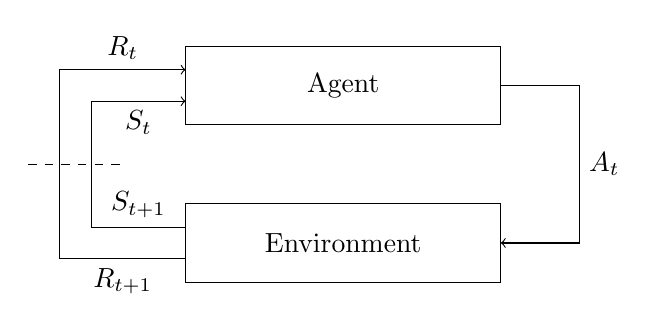
\begin{tikzpicture}
        \draw (0, 2) rectangle node {Agent} (4, 3);
        \draw (0, 0) rectangle node {Environment} (4, 1);

        \draw [->] (4, 2.5) -- (5, 2.5) -- node[right] {$A_t$} (5, 0.5) -- (4, 0.5);

        \draw [->] (0, 0.3) -- node[below] {$R_{t+1}$} (-1.6, 0.3) -- (-1.6, 2.7) --node[above] {$R_t$}  (0, 2.7);
        \draw [->] (0, 0.7) -- node[above] {$S_{t+1}$} (-1.2, 0.7) -- (-1.2, 2.3) -- node[below] {$S_t$} (0, 2.3);

        \draw [dashed] (-2, 1.5) -- (-0.8, 1.5);
    \end{tikzpicture}
    \caption{The agent-environment feedback loop in a Markov Decision Process.}
    \label{fig:mdp_visualization}
\end{figure}

In a \textit{finite Markov Decision Process} \cite{bible}, the sets of states $\mathscr{S}$, actions $\mathscr{A}(s) : \forall s \in \mathscr{S}$, and rewards $\mathscr{R}$ are all finite. With this constraint, we can create a function $p : \mathscr{S} \times \mathscr{R} \times \mathscr{S} \times \mathscr{A} \to \left[0, 1\right]$ to denote probabilities of state transitions occurring. For example, $p\left(s', r \given s, a\right)$ refers to the probability of seeing state $s'$ and receiving reward $r$ after taking action $a$ in state $s$. This implies that transition probabilities are only dependent on the current state and action, but not on historical information.

Usually, an agent is not supposed to focus solely on choosing the action $A_t$ which results in the highest \textit{immediate reward} $R_{t+1}$. Instead, future rewards should also be taken into consideration. Formally, we define the \textit{return} $G_t$ for timestep $t$, which is the sum of all rewards at subsequent timesteps until the final timestep $T$.
\begin{equation*}
    G_t = R_{t+1} + R_{t+2} + R_{t+3} + ... + R_T
\end{equation*}
Accordingly, an agent shall aim to maximize the expected return at each step. The concept of a final timestep only applies to tasks that have a clearly defined beginning and end, making them repetitive in nature. We call a single cycle of these repetitive tasks \textit{episode}.

For tasks that can potentially continue indefinitely, i.e. $T = \infty$, $G_t$ may also become infinite and can, therefore, no longer be subject to maximization. To avoid this issue, we introduce a \textit{discount rate} (or \textit{discount factor}) $\gamma \in [0, 1]$, and define the \textit{discounted return} as follows:
\begin{equation*}
    G_t^{(\gamma)} = R_{t+1} + \gamma R_{t+2} + \gamma^2 R_{t+3} + ...
        = \sum_{k=t+1}^T \gamma^{k-t-1} R_k
\end{equation*}
The parameter $\gamma$ determines to what extend the agent prefers rewards in the near over those in the far future. As an example, an agent with $\gamma = 0$ is only concerned with the immediate reward, whereas the same agent with $\gamma = 0.99$ will optimize for a large time window of rewards. Choosing $\gamma < 1$ ensures that $G_t$ will never become infinite.

In some cases, it is not realistic that the agent receives the full state of the environment. For instance, a robot with a camera cannot possibly measure all physical properties of its surroundings at all times. While a well defined \textit{latent state} may exist, the agent is only provided with an \textit{observation} produced by this state instead. These types of environments are modeled as \textit{Partially Observable Markov Decision Processes}, or \textit{POMDPs} \cite{bible}.
\subsubsection{Value-Based Methods}
\subsubsection{Policy-Based Methods}
\subsubsection{Actor-Critic Methods}